The third category of inputs for \mocasin is \texttt{sdf3}, which uses the \ac{\SDFFF} framework~\cite{sdf3}.
This framework is based on \ac{TGFF}, adapted to the \ac{SDF} model of computation.
We will discuss \ac{SDF} more in detail in Chapter~\ref{chap:mocs}.
However, for the purposes of benchmarking as discussed here, both \ac{SDF} and task graphs can be considered as special cases of \ac{KPN}.
The random graph generation of the \ac{\SDFFF} framework allows multiple configurations on the types of graphs it generates, controlling the number of actors (processes) as well as the degree of connectivity in the graph, firing rates and execution times of the actors, or if the graph is acycilic.

Random benchmark generation has two main advantages over using fixed benchmarks. The first advantage is the amount of benchmarks, which is virtually unlimited with a random generation approach.
The second advantage is the control over the properties of the benchmarks.
Using \ac{\SDFFF} we can consider precisely what effect the properties of the graph have on the algorithms (e.g. its size, or connectivity), by generating benchmarks which have the desired parameters for the independent variable we are investigating.
The main disadvantage is obvious: random benchmarks are not as realistic as actual benchmarks.
It is not clear if we will find a graph like the one generated by \ac{\SDFFF} in a real-life application.

Since we have both the \ac{CPN} and the \ac{E3S} benchmarks, we will focus our evaluation on those.
Instead of discussing the graph generation in \ac{\SDFFF}, we will discuss random benchmark generation from a different type of graph, \emph{level graphs}\cite{goens_multiprog18}.
The main difference is that for the use-case for level graphs in~\cite{goens_multiprog18} we \textbf{do not} have better, realistic benchmarks we can use instead.

The context for benchmark generation we will discuss here are micro-service-oriented architectures.
Large internet companies like Facebook or Twitter have an infrastructure that consists of multiple micro-services that depend on each other~\cite{marlow2014haxl}.
A crucial factor for optimal performance is the amount of \ac{I/O} calls these micro-services make.
We will discuss the use case more in-depth in Chapter~\ref{chap:pl}. 
In this section we will only focus on the benchmark generation.

The micro-service-based infrastructures from large companies like Facebook or Twitter are the \acf{IP} of these companies and not in the public domain.
If, for example, we want to improve and compare a method for optimizing \ac{I/O} in Facebook's spam-fighting service~\cite{marlow2014haxl}, we cannot use a large representative benchmark sample from Facebook to test against their method.
Instead, we observe the general structure of the programs in their work and device a methodology for generating random benchmarks, with a method we call level graphs~\cite{goens_multiprog18}.

\begin{figure*}[th]
	\centering
	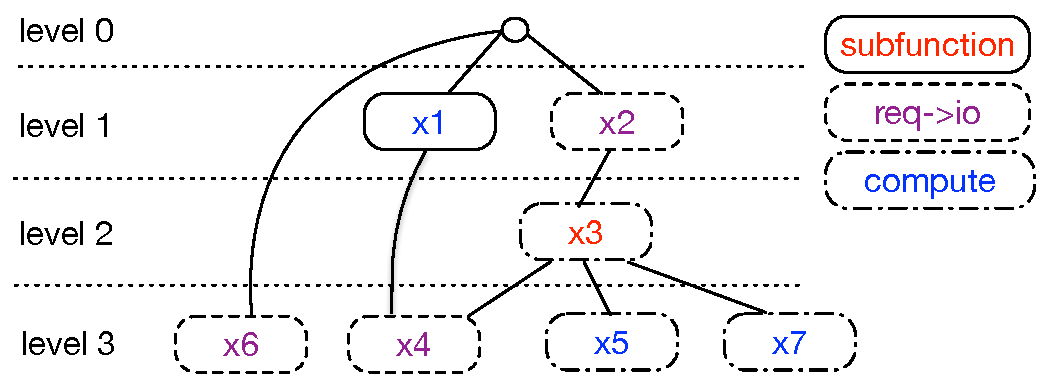
\includegraphics[width=\textwidth]{figures/level-graph.pdf}
	\caption{An example of a Level Graph. Reproduced from Figure~1 of \cite{goens_multiprog18}.}
	\label{fig:level_graph}
\end{figure*}

Figure~\ref{fig:level_graph} shows an example of a level graph. The graph depicted is a tree which is organized by levels, which are indexed with integer numbers.
The nodes in the graph are labeled as different kinds of node, namely \texttt{req$\rightarrow$io},\texttt{subfunction} and \texttt{compute}.
The graph depicted is designed to benchmark \ac{I/O} optimization, which is why the node labels are designed accordingly, reflecting \ac{I/O} calls and other computation,
as well as an additional \texttt{subfunction} node that creates nested benchmarks with additional function calls.
This is also by design, to test the use-case.

The idea behind level graphs is to reflect the intuition of \emph{locality} in code\index{locality in code}.
This intuition is based on the observation that long-rage dependencies in code are less common than short-ranged ones.
While programmers do sometimes refer back to identifiers defined far behind, it is far more common to define values before using them.
We interpret this as a statistical feature of the distribution of code as commonly written by humans (cf. Section~\ref{sec:representative_benchmarks}).
Levels in level graphs are thus designed to define the probability distribution of dependencies in graphs.

There are generally two accepted and common models of random graphs, the Erd\H{o}s-R\'{e}yni approach~\cite{erdosreyni} and the Gilbert approach~\cite{gilbert1959random}.
The former defines a uniform distribution over all graphs for a given number of nodes, while the latter defines the probabilities of the edges independently.
Our definition of \emph{Level Graphs}\index{level graph} is based on the Gilbert approach, but instead of having uniform probabilities, the probabilities are defined through the levels.
Concretely, a level graph $L = ((V,E),l)$ is a directed graph $(V,E)$ with a level function $l : V \rightarrow \mathbb{N}$ to the natural numbers, with the property that for all nodes $v,w \in V$ there can only be an edge $(v,w) \in E$ if the level of $v$ is smaller than that of $w$, i.e. $(v,w) \in E \Rightarrow l(v) < l(w)$.
To generate a probability distribution in level graphs we define the probability of the edge $(v,w) \in E$ to be as follows:
\[  p( (v,w) ) = \left\{
    \begin{array}{ll}
      0, & \text{ if } l(v) \geq l(w), \\
      2^{l(v)-l(w)}, & \text{ otherwise.}
    \end{array} \right. \]
The method can be generalized by choosing a different probability for the case where $l(v) < l(w)$.
The chosen value $2^{l(v)-l(w)}$ is, to an extent, arbitrary.
This probability definition ensures that dependencies are more common locally, between levels that are close by, discouraging but not prohibiting long-range dependencies.

A level graph can be used to generate code in different languages or back-ends, expressing the same computation.
In~\cite{goens_multiprog18} we implemented three back-ends for \ac{I/O} optimizing frameworks, one for Ohua/\"{Y}auhau~\cite{ertel_cc18} (see Section~\ref{sec:yauhau}), one for Twitter's Muse~\cite{muse} and one for Facebook's Haxl~\cite{marlow2014haxl}.
These back-ends are also based on different languages, namely Clojure and Haskell.
The abstract nature of level graphs allows us to generate code in different languages.